\section{Results}\label{sec:results}
\subsection{Proving and Verifying Times}\label{subsec:results:provingverifying}
\begin{figure*}[!htb]
    \centering
    \subfloat[\centering Proving Time]{{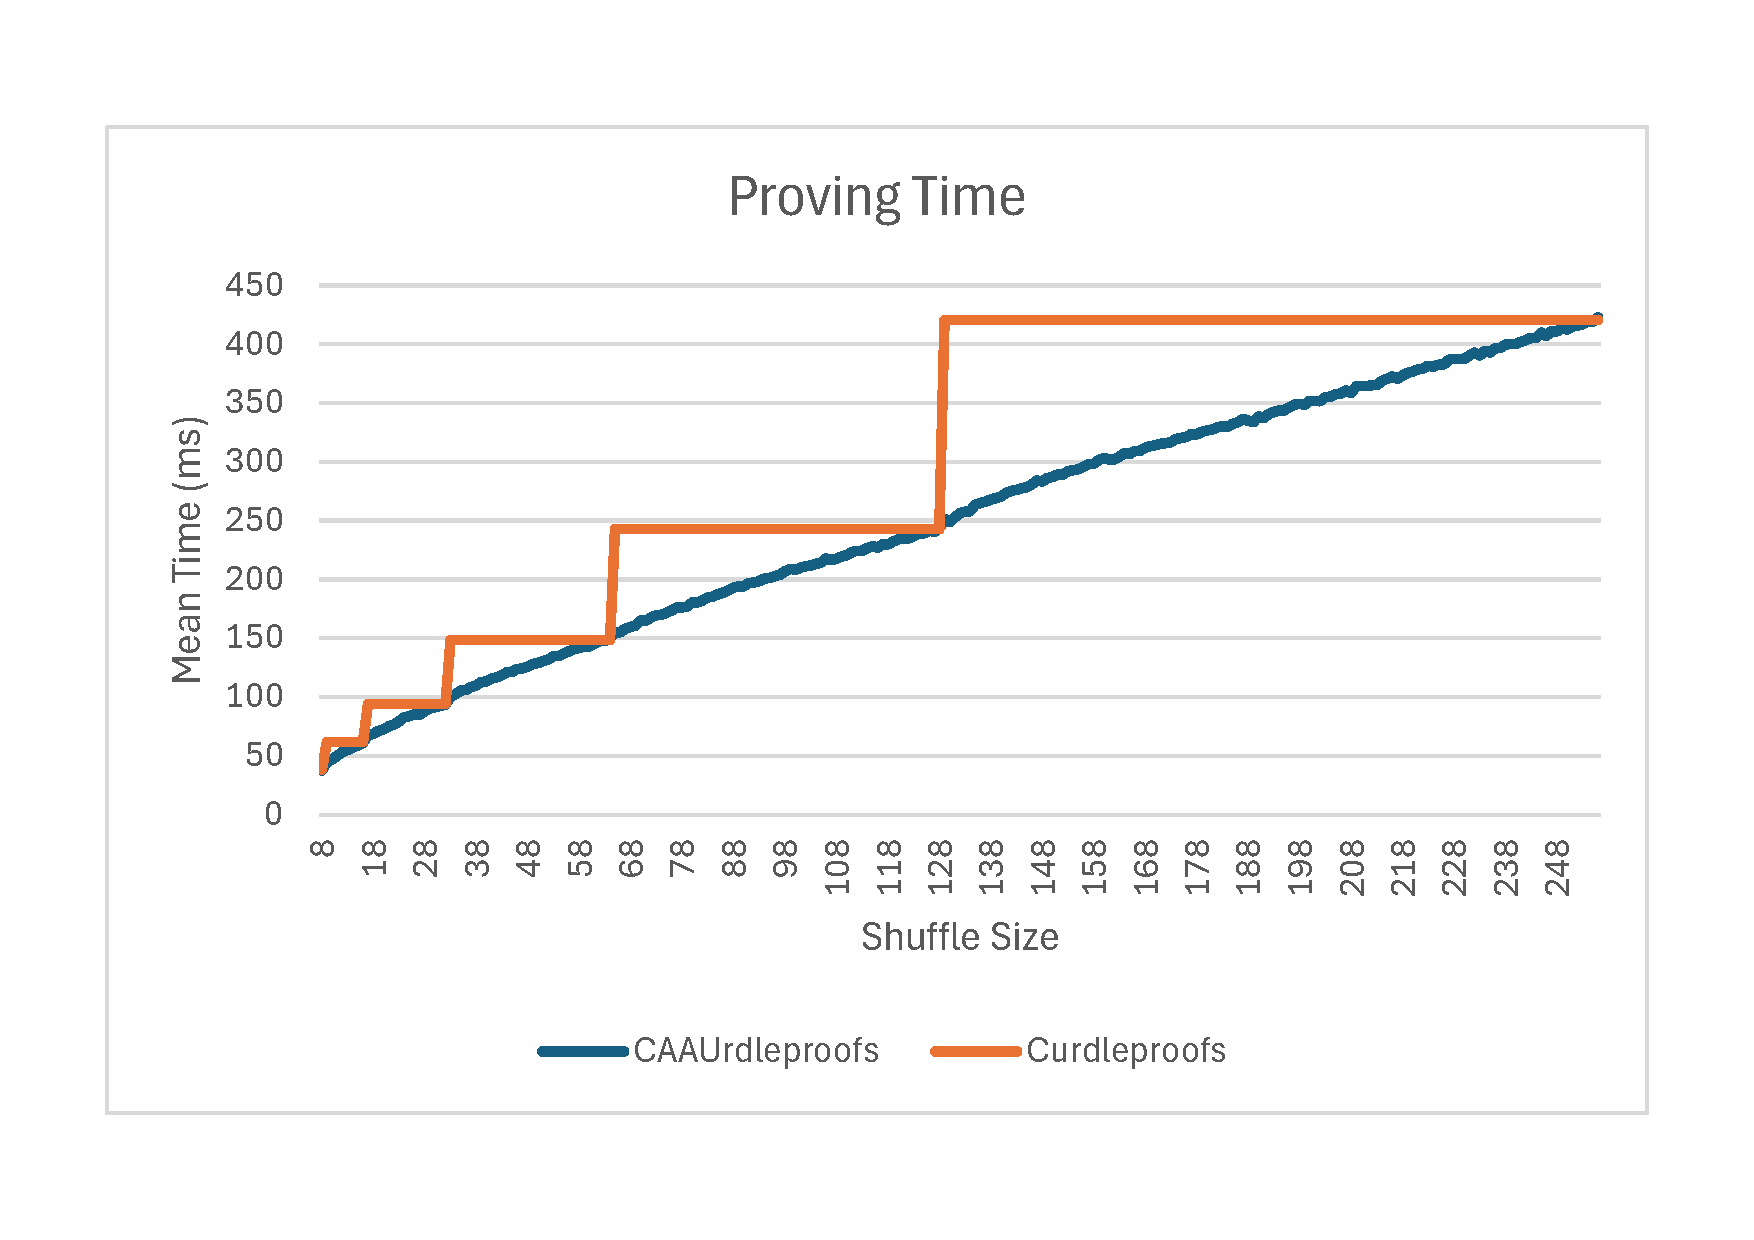
\includegraphics[width=0.45\textwidth]{figures/results/provingtime} }}%
    \qquad
    \subfloat[\centering Verifying Time]{{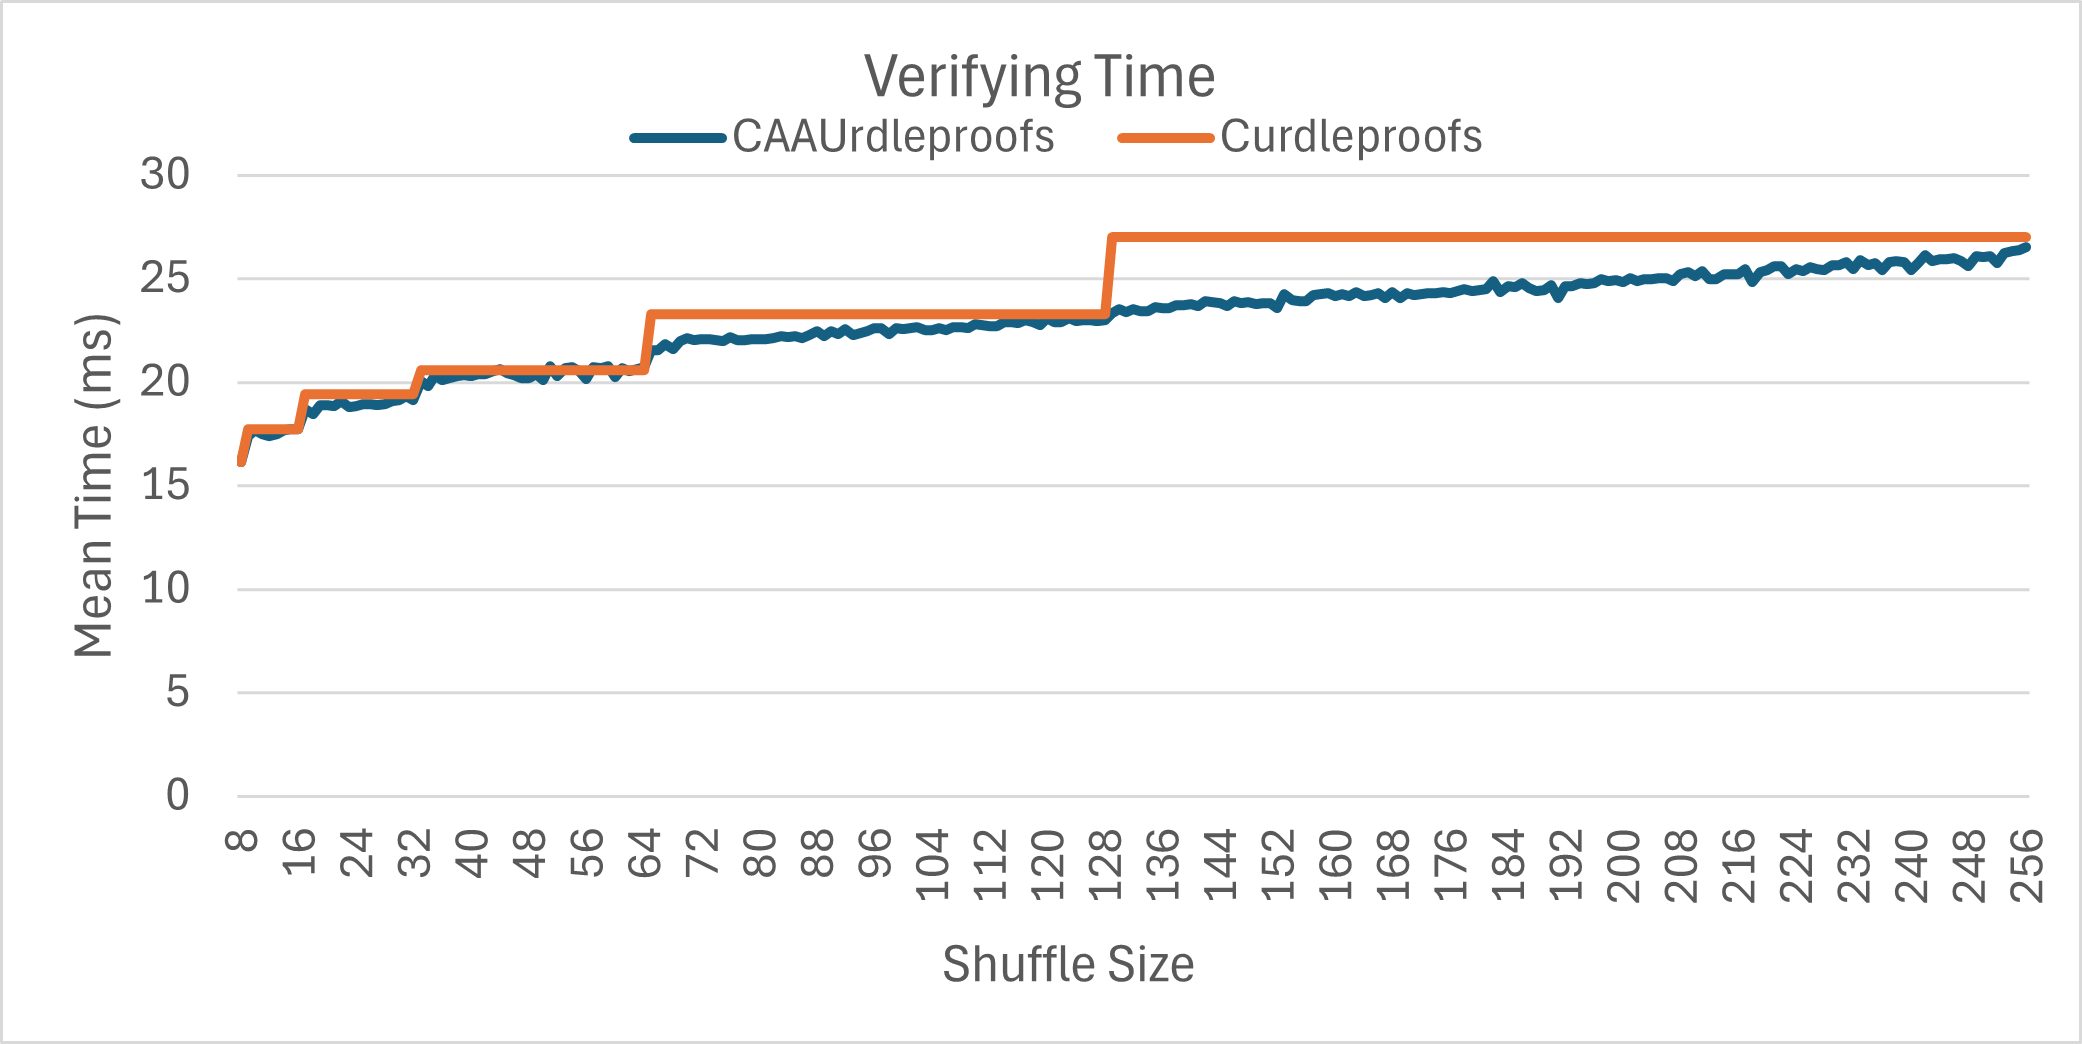
\includegraphics[width=0.45\textwidth]{figures/results/verifyingtime} }}%
    \caption{The timed results compared between CAAUrdleProofs and Curdleproofs}%
    \label{fig:resulttimes}%
\end{figure*}
After running the experiment where Curdleproofs and CAAUrdleproofs were compared across different Shuffle sizes, we obtained the results shown in \autoref{fig:resulttimes}.
As mentioned in \autoref{sec:CAAUrdleproof-experiment}, CAAUdleproofs was run with a shuffle size $k$ of $\{8,9,\dots,256\}$ but Curdleproofs was only run with a shuffle size $k$ of $\{8,16,32,64,128,256\}$.
This is why the results for Curdleproofs instantly goes up to the next size of $k$ because it would have to pad the inputset until it reaches the next size of a power of 2.
From the results, we can see that CAAUrdleproofs and Curdleproofs have similar proving and verifying times when $k$ is a power of 2 but whenever $k$ is not a power of 2 CAAUrdleproofs is faster.


\subsection{Shuffle security}\label{subsec:Shuffle-security}

